\documentclass[a4paper, 12pt]{article}

\usepackage[top=2cm, bottom=3cm, right=2cm, left=2cm]{geometry}
\usepackage[utf8]{inputenc}
\usepackage{amsmath, amsfonts, amssymb}
\usepackage{float}
\usepackage{graphicx}
\usepackage[portuguese]{babel}

\title{Cálculo Diferencial e Integral 2

Lista 3}
\author{
Igor Galdeano Rodrigues - SP3037223
\\
Luís Otávio Lopes Amorim - SP3034178}

\newcommand{\solucao}{\begin{center}\textbf{SOLUÇÃO}\end{center}}
\DeclareMathOperator{\sen}{sen}


\begin{document}
	\maketitle
	\begin{enumerate}
		\item Na figura abaixo, estão representadas as curvas de nível (ou o diagrama de
contornos) de uma função de duas variáveis. Em relação a elas, marque a alternativa ou
alternativas que contenham as duas afirmações verdadeiras: 

\begin{center}
	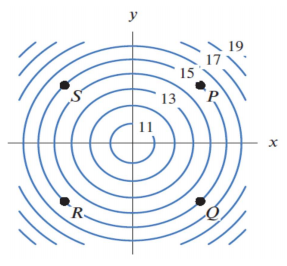
\includegraphics[scale=1]{fig1}
\end{center}

\begin{enumerate}
	\item $f_x(S) < 0$ e $f_y(R) > 0$
	\item $f_x(S) < 0$ e $f_y(R) > 0$
	\item $f_x(S) < 0$ e $f_y(R) > 0$
	\item $f_x(S) < 0$ e $f_y(R) > 0$
	\item $f_x(S) < 0$ e $f_y(R) > 0$
\end{enumerate}

\solucao

A única alternativa correta é a letra a.

		\pagebreak
		\item Considere as funções $f(x,y) = x \cdot e^{x^2 - y^2}$
e $g(x, y) = \ln{\frac{1}{\sqrt{x^2+y^2}}}$. Sobre estas
funções, marque a alternativa ou alternativas que contenham
duas afirmações verdadeiras.

\begin{enumerate}
	\item $f_y(x, y) = -2y \cdot e^{x^2-y^2}$ e $g_{xy}(x, y) + g_{yx}(x,y) = 0 $
	\item $f_{yx}(x, y) = -2y \cdot (1+2x^2) \cdot e^{x^2-y^2}$ e $g_{xx}(x, y) + g_{yy}(x,y) = 0 $
	\item $f_x(x, y) = (1+2x^2) \cdot e^{x^2-y^2}$ e $g_{xx}(x, y) - g_{yy}(x,y) = 0 $
	\item $f_y(x, y) = -2xy \cdot e^{x^2 - y^2}$ e $g_{xy}(x, y) - g_{yx}(x,y) = 0 $
	\item $f_{xy}(x, y) = -2y \cdot (1+2x^2) \cdot e^{x^2-y^2}$ e $g_{xx}(x, y) + g_{yy}(x,y) = 0 $
\end{enumerate}

Calculando cada uma das derivadas parciais obtivemos:
		
\solucao
\begin{center}
$
\begin{array}{ccc}
	\dfrac{\partial f}{\partial y} = x \cdot e^{(x^2 - y^2)} &
	\dfrac{\partial f}{\partial x} = e^{(x^2-y^2)}(1+2x^2) &
	\dfrac{\partial^2 f}{\partial y \partial x} = -2y(1+2x^2)e^{(x^2-y^2)} \\ \\
	\dfrac{\partial^2 g}{\partial x^2} = \dfrac{x^2 - y^2}{(x^2+y^2)^2} &
	\dfrac{\partial^2 g}{\partial y^2} = \dfrac{y^2 - x^2}{(x^2+y^2)^2} &
	\dfrac{\partial^2 g}{\partial x \partial y} = \dfrac{2xy}{(x^2+y^2)^2}
\end{array}
$
\end{center}

Com isso, analisando as alternativas, apenas as letras
$b$, $d$ e $e$ apresentam duas afirmações corretas.
		\item
Utilizando a fórmula deforça com corrente:

$$
F = i \cdot L \cdot B \cdot \sin \theta
$$

Reorganizando a fórmula temos:

$$
L = \frac{F}{i B \sin \theta}
$$

Substituindo os valores:

$$
L = \frac{3,5 \cdot 10^{-3}}{6 \cdot 2 \cdot 0,642}
$$

$$
L \approx 453,75m
$$
		\\ \\ \\
\item Seja $w = f(x, y)$, onde f é uma função diferenciavel.
Se $x = r \cos \theta$ e $y = r \sen \theta$, quais das
afirmações abaixo são verdadeiras (pode haver mais de uma)?

Sugestão: neste exercício você deve usar a regra da cadeia.

\begin{enumerate}
	\item $\left(\dfrac{\partial w}{\partial r}\right)^2 +
			\left(\dfrac{\partial w}{\partial \theta}\right)^2
			= \left(\dfrac{\partial w}{\partial x}\right)^2 + \dfrac{1}{r^2} \cdot
			\left(\dfrac{\partial w}{\partial y}\right)^2$
	
	\item $\left(\dfrac{\partial w}{\partial x}\right)^2 -
			\left(\dfrac{\partial w}{\partial y}\right)^2
			= \left(\dfrac{\partial w}{\partial r}\right)^2 - \dfrac{1}{r^2} \cdot
			\left(\dfrac{\partial w}{\partial \theta}\right)^2$
			
	\item $\left(\dfrac{\partial w}{\partial r}\right)^2 +
			\left(\dfrac{\partial w}{\partial \theta}\right)^2
			= \left(\dfrac{\partial w}{\partial x}\right)^2 + r^2 \cdot
			\left(\dfrac{\partial w}{\partial y}\right)^2$
			
	\item $\left(\dfrac{\partial w}{\partial x}\right)^2 +
			\left(\dfrac{\partial w}{\partial y}\right)^2
			= \left(\dfrac{\partial w}{\partial r}\right)^2 + \dfrac{1}{r^2} \cdot
			\left(\dfrac{\partial w}{\partial \theta}\right)^2$
	
	\item $\left(\dfrac{\partial w}{\partial r}\right)^2 +
			\left(\dfrac{\partial w}{\partial y}\right)^2
			= \left(\dfrac{\partial w}{\partial x}\right)^2 + \dfrac{1}{r^2} \cdot
			\left(\dfrac{\partial w}{\partial \theta}\right)^2$
\end{enumerate}

\solucao

Inicialmente calculamos as derivadas parciais de
$w$ em relação a $r$ e $\theta$.

\begin{center}
$$
\begin{array}{c}
	\dfrac{\partial w}{\partial r} =
	\dfrac{\partial w}{\partial x} \cos \theta +
	\dfrac{\partial w}{\partial y} \sen \theta \\ \\
	\dfrac{\partial w}{\partial \theta} =
	-\dfrac{\partial w}{\partial x} r \sen \theta +
	\dfrac{\partial w}{\partial y} r \cos \theta
\end{array}
$$
\end{center}

Em seguida, elevamos ambas as derivadas ao quadrado obtendo:

\begin{center}
$$
\begin{array}{c}
	\left(\dfrac{\partial w}{\partial r}\right)^2 =
	\left(\dfrac{\partial w}{\partial x}\right)^2 \cos ^2 \theta +
	\left(\dfrac{\partial w}{\partial y}\right)^2 \sen ^2 \theta +
	2 \dfrac{\partial w}{\partial x} \dfrac{\partial w}{\partial y}
	\cos \theta \sen \theta \\ \\
	\left(\dfrac{\partial w}{\partial \theta}\right)^2 =
	\left(\dfrac{\partial w}{\partial x}\right) r^2 \sen ^2 \theta +
	\left(\dfrac{\partial w}{\partial y}\right) r^2 \cos ^2 \theta - 
	2r^2 \dfrac{\partial w}{\partial x} \dfrac{\partial w}{\partial y}
	\cos \theta \sen \theta
\end{array}
$$
\end{center}

Observando as alternativas, podemos perceber que se resumem
a 3 somas: $f_r^2+f_{\theta}^2$, $f_r^2+\dfrac{1}{r^2}f_{\theta}^2$ e
$f_r^2-\dfrac{1}{r^2}f_{\theta}^2$, realizando elas, chegamos aos resultados:

$$
\left( \dfrac{\partial w}{\partial r}\right)^2 +
\left( \dfrac{\partial w}{\partial \theta}\right)^2 = 
\left( \dfrac{\partial w}{\partial x}\right)^2
(\cos \theta + r^2 \sen \theta) +
\left( \dfrac{\partial w}{\partial y}\right)^2
(\sen \theta + r^2 \cos \theta) +
2r\dfrac{\partial w}{\partial x} \dfrac{\partial w}{\partial y}
\sen \theta \cos \theta (1 - r^2)
$$ 

$$
\left( \dfrac{\partial w}{\partial r}\right)^2 +
\dfrac{1}{r^2}\left( \dfrac{\partial w}{\partial \theta}\right)^2 =
\left( \dfrac{\partial w}{\partial x}\right)^2 +
\left( \dfrac{\partial w}{\partial y}\right)^2
$$

$$
\left( \dfrac{\partial w}{\partial r}\right)^2 -
\dfrac{1}{r^2}\left( \dfrac{\partial w}{\partial \theta}\right)^2 =
\left( \dfrac{\partial w}{\partial x}\right)^2
\cos (2\theta) -
\left( \dfrac{\partial w}{\partial y}\right)^2
\cos (2\theta) +
4\dfrac{\partial w}{\partial x} \dfrac{\partial w}{\partial y}
\sen \theta \cos \theta
\
$$

Desta forma, a única alternativa correta é a letra d.
		\item Calcular os autovalores e autovetores das
seguintes matrizes

\begin{enumerate}
	%	LETRA A 	%
	\item 
	$A = 
	\begin{bmatrix}
		 1 & 3 \\
		-1 & 5
	\end{bmatrix}		
	$
	\pagebreak
	\solucao
	$$det
	\begin{bmatrix}
		 1 - \lambda & 3 \\
		-1           & 5 - \lambda
	\end{bmatrix}
	=
	(1 - \lambda)(5-\lambda) + 3	
	=
	\lambda^2 - 6\lambda+8 = 0	
	$$
	$$
	\Delta = 6^2 - 4\cdot 1 \cdot 8 = 4
	\lambda = \frac{6 \pm \sqrt{4}}{2}
	$$
	\begin{center}
	$\lambda_1 = 2$
	$\lambda_2 = 4$	
	\end{center}
	Agora, encontrando os autovetores:
	
	$$
	\begin{pmatrix}
		-1 & 3 \\
		-1 & 3
	\end{pmatrix}
	x = 3y
	\, \, \, 
	v_1 = (3, \, 1)
	$$
	
	$$
	\begin{pmatrix}
		-3 & 3 \\
		-1 & 1
	\end{pmatrix}
	x = y
	\, \, \, 
	v_2 = (1, \, 1)
	$$
	
	Portanto, temos:
	
	$$
	\begin{array}{cc}
		\lambda_1 = 2 & \lambda_2 = 4 \\
		v_1 = (3, \, 1) & v_2 = (1, \, 1)
	\end{array}		
	$$
	
	%	LETRA B 	%
	\item
	$A = 
	\begin{bmatrix}
		3 &  3 & -1 \\
		0 & -1 &  0 \\
		8 &  6 & -5
	\end{bmatrix}		
	$
	\\ \\
	\solucao
	$$det
	\begin{pmatrix}
		3 - \lambda &  3           & -1           \\
		0           & -1 - \lambda &  0           \\
		8           &  6           & -5 - \lambda 
	\end{pmatrix}
	= (3 - \lambda)
	\begin{vmatrix}
		-1 - \lambda & 0           \\
		 6           & -5 - \lambda
	\end{vmatrix}
	-3
	\begin{vmatrix}
		0 &  0           \\
		8 & -5 - \lambda
	\end{vmatrix}
	-2
	\begin{vmatrix}
		0 & -1 - \lambda \\
		8 &  6          
	\end{vmatrix}
	$$
	\\
	\begin{center}
		$
		(3 - \lambda)(1+\lambda)(5+\lambda) - 16(1+\lambda) =
		(1+\lambda)\left[(3-\lambda)(5+\lambda) - 16\right]=0		
		$
		
		$
		(1+\lambda)(-\lambda^2-2\lambda-1) =
		-(1+\lambda)(\lambda^2+2\lambda+1) = -(1+\lambda)^3 = 0 \Rightarrow \lambda = -1$
	\end{center}
	
	Portanto, temos apenas um valor $\lambda = 1$ com multiplicidade 3.
	Procurando os autovetores:
	
	$$
	\begin{pmatrix}
		4 & 3 & -2 & 0\\
		0 & 0 &  0 & 0\\
		8 & 6 & -4 & 0
	\end{pmatrix}
	\begin{array}{c}
		\\ \\ L_3 = L_3 - 2L_1
	\end{array}
	\begin{pmatrix}
		4 & 3 & -2 & 0\\
		0 & 0 &  0 & 0\\
		0 & 0 &  0 & 0
	\end{pmatrix}
	4x+3y-2z = 0
	$$
	Isolando $x$ na equação encontrada, podemos encontrar
	a base do plano que determina o auto-esaço da matriz.
	$$
	x = -\frac{3y}{4} + \frac{z}{2}	
	$$
	$$
	(x, \, y, \, z) = y(-3, \, 4, \, 0) + z(1, \, 0, \, 2)	
	$$
	
	Desta base, podemos tirar os autovetores:
	
	$$
	\begin{array}{ccc}
		& \lambda = -1 & \\
		v_1 = (-3, \, 4, \, 0) & & v_2 = (1, \, 0, \, 2)
	\end{array}		
	$$
	
	
\end{enumerate}
		\item Determinar uma matriz P que diagonaliza A
e calcular $P^{-1}AP$. Calcule $A^{30}$ e $B^{101}$.

\begin{enumerate}
	%	LETRA A 	%
	\item
	$
	\begin{bmatrix}
		0 &  0 & 2 \\
		0 & -1 & 0 \\
		2 &  0 & 0
	\end{bmatrix}
	$
	\\ \\
	\solucao
	$$
	det 
	\begin{pmatrix}
		-\lambda &  0 & 2 \\
		0        & -1 - \lambda & 0 \\
		2 &  0 & - \lambda
	\end{pmatrix}
	= -\lambda
	\begin{vmatrix}
		-1 -\lambda & 0 \\
		0 & -\lambda
	\end{vmatrix}
	-0
	\begin{vmatrix}
		0 & 0 \\
		2 & -\lambda
	\end{vmatrix}
	+2
	\begin{vmatrix}
		0 & -1 -\lambda \\
		2 & 0
	\end{vmatrix}
	$$

	$$-\lambda^2(1+\lambda)+4(1+\lambda) = (1+\lambda)(4-\lambda^2) = 0$$
	
	$$
	\begin{array}{ccc}
		\lambda_1 = -2 & \lambda_2 = -1 & \lambda_3 = 2
	\end{array}
	$$
	
	Agora, basta encontrar os autovetores.
	
	$$
	\begin{pmatrix}
		2 & 0 & 2 & 0 \\
		0 & 1 & 0 & 0 \\
		2 & 0 & 2 & 0
	\end{pmatrix}		
	\begin{array}{c}
		x = -z \\
		y = 0 \\
	\end{array}		
	v_1 = (1, \, 0, \, -1)	
	$$
	
	$$
	\begin{pmatrix}
		1 & 0 & 2 & 0 \\
		0 & 0 & 0 & 0 \\
		2 & 0 & 1 & 0
	\end{pmatrix}		
	\begin{array}{c}
		\\ \\ L_3 = 2L_3 - L_1
	\end{array}	
	\begin{pmatrix}
		1 & 0 & 2 & 0 \\
		0 & 0 & 0 & 0 \\
		3 & 0 & 0 & 0
	\end{pmatrix}
	\begin{array}{c}
		z = 0 \\
		\\
		x = 0
	\end{array}	
	v_2 = (0, \, 1, \, 0)	
	$$
	
	$$
	\begin{pmatrix}
		-2 & 0 & 2 & 0 \\
		0 & -3 & 0 & 0 \\
		2 & 0 & -2 & 0
	\end{pmatrix}		
	\begin{array}{c}
		L_1 = \frac{L_1}{2} \\
		\\
		L_3 = L_1 + L_3
	\end{array}	
	\begin{pmatrix}
		-1 & 0 & 1 & 0 \\
		0 & -3 & 0 & 0 \\
		0 & 0 & 0 & 0
	\end{pmatrix}
	\begin{array}{c}
		x = z \\
		y = 0
	\end{array}	
	v_3 = (1, \, 0, \, 1)	
	$$
	
	A matriz $P$ é a matriz cujas colunas
	são os autovetores de $A$, ou seja, 
	$P = \begin{bmatrix}
		1 & 0 & 1 \\
		0 & 1 & 0 \\
		-1 & 0 & 1
	\end{bmatrix}
	$. Para encontrar $P^{-1}$ basta transformar
	$P$ em $I$ ao lado da matri $I$:
	
	$$
	\begin{pmatrix}
		1  & 0 & 1 & 1 & 0 & 0\\
		0  & 1 & 0 & 0 & 1 & 0\\
		-1 & 0 & 1 & 0 & 0 & 1
	\end{pmatrix}
	\begin{array}{c}
		L_1 = \frac{L_1-L_3}{2} \\ \\
		L_3 = \frac{L_1 + L_3}{2}
	\end{array}
	\begin{pmatrix}
		1 & 0 & 0 & \frac{1}{2} & 0 & -\frac{1}{2}\\
		0 & 1 & 0 & 0 & 1 & 0\\
		1 & 0 & 1 & \frac{1}{2} & 0 & \frac{1}{2}
	\end{pmatrix}
	$$
	
	Desta forma, $P^{-1} = 
	\begin{pmatrix}
		\frac{1}{2} & 0 & -\frac{1}{2}\\
		0 & 1 & 0\\
		\frac{1}{2} & 0 & \frac{1}{2}
	\end{pmatrix}$, com isso podemos calcular $P^{-1}AP$ e checar
	que esta matriz é a matriz cuja diagonal principal são os autovalores de $A$
	e o resto dos valores são todos nulos.
	
	$$
	P^{-1}AP = 
	\begin{pmatrix}
		\frac{1}{2} & 0 & -\frac{1}{2}\\
		0 & 1 & 0\\
		\frac{1}{2} & 0 & \frac{1}{2}
	\end{pmatrix}
	\begin{pmatrix}
		0 & 0 & 2\\
		0 & -1 & 0\\
		2 & 0 & 0
	\end{pmatrix}
	\begin{pmatrix}
		1 & 0 & 1\\
		0 & 1 & 0\\
		-1 & 0 & 1
	\end{pmatrix}
	=
	\begin{pmatrix}
		-1 & 0 & 1\\
		0 & -1 & 0\\
		1 & 0 & 1
	\end{pmatrix}
	\begin{pmatrix}
		1 & 0 & 1\\
		0 & 1 & 0\\
		-1 & 0 & 1
	\end{pmatrix}
	$$
	
	$$
	P^{-1}AP =
	\begin{pmatrix}
		-2 & 0 & 0\\
		0 & 1 & 0\\
		0 & 0 & 2
	\end{pmatrix}
	=
	\begin{pmatrix}
		\lambda_1 & 0 & 0\\
		0 & \lambda_2 & 0\\
		0 & 0 & \lambda_3
	\end{pmatrix}
	$$
	
	Finalmente, utilizarei a matri diagonalizada para
	calcular $A^{30}$. Isso pois, multiplicações com
	matrizes diagonalizadas são muito mais fáceis.
	Além disso, sendo $D$ a matriz $A$ diagonalizada, da
	relação $D = P^{-1}AP$, podemos encontrar $A = PDP{-1}$.
	Portanto, após encontrar $D^{30}$, encontrar $A^{30}$ é um processo fácil.
	
	$$
	D^2 = 
	\begin{pmatrix}
		-2 & 0 & 0\\
		0 & 1 & 0\\
		0 & 0 & 2
	\end{pmatrix}
	\begin{pmatrix}
		-2 & 0 & 0\\
		0 & 1 & 0\\
		0 & 0 & 2
	\end{pmatrix}
	=
	\begin{pmatrix}
		4 & 0 & 0\\
		0 & 1 & 0\\
		0 & 0 & 4
	\end{pmatrix}	
	$$
	
	$$
	D^3 = 
	\begin{pmatrix}
		4 & 0 & 0\\
		0 & 1 & 0\\
		0 & 0 & 4
	\end{pmatrix}
	\begin{pmatrix}
		-2 & 0 & 0\\
		0 & 1 & 0\\
		0 & 0 & 2
	\end{pmatrix}
	=
	\begin{pmatrix}
		-8 & 0 & 0\\
		0 & 1 & 0\\
		0 & 0 & 8
	\end{pmatrix}	
	$$
	Com isso, podemos perceber que elevar uma matriz diagonalizada
	a um número n é o mesmo que elevar os valores de sua diagonal
	principal a n, assim::
	
	$$
	D^{30} = 
	\begin{pmatrix}
		(-2)^{30} & 0 & 0\\
		0 & 1 & 0\\
		0 & 0 & 2^{30}
	\end{pmatrix}$$
	
	Por fim, basta encontrar $A^{30}$
	
	$$
	A^{30} = PD^{30}P^{-1}
	=
	\begin{pmatrix}
		1 & 0 & 1\\
		0 & 1 & 0 \\
		-1 & 0 & 1 
	\end{pmatrix}
	\begin{pmatrix}
		(-2)^{30} & 0 & 0\\
		0 & 1 & 0\\
		0 & 0 & 2^{30}
	\end{pmatrix}
	\begin{pmatrix}
		\frac{1}{2} & 0 & -\frac{1}{2}\\
		0 & 1 & 0\\
		\frac{1}{2} & 0 & \frac{1}{2}
	\end{pmatrix}
	$$
	
	$$
	A^{30} = 
	\begin{pmatrix}
		2^{30} & 0 & 2^{30} \\
		0 & 1 & 0 \\
		-2^{30} & 0 & 2^{30}
	\end{pmatrix}
	\begin{pmatrix}
		\frac{1}{2} & 0 & -\frac{1}{2}\\
		0 & 1 & 0\\
		\frac{1}{2} & 0 & \frac{1}{2}
	\end{pmatrix}
	=
	\begin{pmatrix}
		2^{30} & 0 & 0 \\
		0 & 1 & 0 \\
		0 & 0 & 2^{30}
	\end{pmatrix}
	$$
	
	Desta forma, temos como respostas:
	
	$$
	\begin{array}{ccc}
		P = 
		\begin{pmatrix}
			1 & 0 & 1 \\
			0 & 1 & 0 \\
			-1 & 0 & 1
		\end{pmatrix}
		&
		P^{-1}AP = 
		\begin{pmatrix}
			-2 & 0 & 0 \\
			0 & -1 & 0 \\
			0 & 0 &  2
		\end{pmatrix}
		&
		A^{30} = 
		\begin{pmatrix}
			1073741824 & 0 & 0 \\
			0 & 1 & 0 \\
			0 & 0 & 1073741824
		\end{pmatrix}
	\end{array}				
	$$
	
	%	LETRA B 	%
	\pagebreak
	\item
	$
	\begin{bmatrix}
		2 &  -2 & 1 \\
		-2 & 2 & 1 \\
		-1 &  1 & 5
	\end{bmatrix}
	$
	\\ \\
	\solucao
	
	$$
	det
	\begin{pmatrix}
		 2 - \lambda &  -2 & 1 \\
		-2 & 2 - \lambda & 1 \\
		-1 &  1 & 5 - \lambda
	\end{pmatrix}
	=
	(2 - \lambda)
	\begin{vmatrix}
		2 - \lambda & 1 \\
		1 & 5 - \lambda	
	\end{vmatrix}
	+ 2
	\begin{vmatrix}
		-2 & 1 \\
		-1 & 5 - \lambda
	\end{vmatrix}
	- 1
	\begin{vmatrix}
		-2 & 2 - \lambda \\
		-1 & 1
	\end{vmatrix}
	$$
	
	$$(2 - \lambda)(\lambda^2 - 7\lambda+9)+2(2\lambda-9)+\lambda = 0$$
	
	$$\lambda^3 - 9\lambda^2 - 18\lambda = \lambda(\lambda^2 -9\lambda-18) = 0$$
		
	$$
	\begin{array}{cc}
		\Delta = 81 - 72 = 9 & \lambda = \dfrac{9 \pm 3}{2}
	\end{array}	
	$$

	$$
	\begin{array}{ccc}
		\lambda_1 = 0 & \lambda_2 = 3 & \lambda = 6
	\end{array}
	$$
	
	Agora encontrando os autovetores:
	
	$$
	\begin{pmatrix}
		2 &  -2 & 1 & 0\\
		-2 & 2 & 1 & 0\\
		-1 &  1 & 5 & 0
	\end{pmatrix}	
	\begin{array}{c}
		\\ L_2 = L_2 + L_1 \\ L_3 = 2L_3 + L_1
	\end{array}
	\begin{pmatrix}
		2 &  -2 & 1 & 0\\
		0 & 0 & 0 & 0\\
		0 & 0 & 9 & 0
	\end{pmatrix}
	\begin{array}{cc}
		x = y\\ & v_1 = (1, \, 1, \, 0) \\ z = 0
	\end{array}
	$$
	
	$$
	\begin{pmatrix}
		-1 &  -2 & 1 & 0\\
		-2 & -1 & 1 & 0\\
		-1 &  1 & 2 & 0
	\end{pmatrix}	
	\begin{array}{c}
		\\ L_2 = L_2 + L_1 \\ L_3 = L_3 + 2L_1
	\end{array}
	\begin{pmatrix}
		-1 & -2 & 1 & 0\\
		-3 & -3 & 0 & 0\\
		-3 & -3 & 0 & 0
	\end{pmatrix}
	\begin{array}{c}
		-x-2y-z=0 \Rightarrow y = -z \\ x = -y \\ v_2 = (1, \, -1, \, 1)
	\end{array}
	$$

	$$
	\begin{pmatrix}
		-4 &  -2 & 1 & 0\\
		-2 & -4 & 1 & 0\\
		-1 &  1 & -1 & 0
	\end{pmatrix}	
	\begin{array}{c}
		L_1 = - L_3\\ L_2 = L_2 - 2L_3 \\ L_3 = L_1 -4 L_3
	\end{array}
	\begin{pmatrix}
		1 & -1 & 1 & 0\\
		0 & -6 & 3 & 0\\
		0 & -6 & 3 & 0
	\end{pmatrix}
	\begin{array}{c}
		x-y+z=0 \Rightarrow x = -y \\ z = 2y \\ v_3 = (1, \, -1, \, -2)
	\end{array}
	$$
	
	Encontrados os três autovetores, podemos escrever a matriz $P$,
	colocando cada um dos autovetores em uma coluna, assim 
	$P = 
	\begin{pmatrix}
		1 & 1 & 1 \\
		1 & -1 & -1 \\
		0 & 1 & -2
	\end{pmatrix}
	$. Com isso, podemos encontrar $P^{-1}$ e verificar que
	$P^{-1}BP$ é uma matriz cuja diagonal principal são os autovalores
	de $B$ e os outros elementos são nulos.
	
	$$
	\begin{pmatrix}
		1 & 1 & 1  & 1 & 0 & 0\\
		1 & -1 & -1 & 0 & 1 & 0\\
		0 & 1 & -2 & 0 & 0 & 1
	\end{pmatrix}
	\begin{array}{c}
		L_1 = \dfrac{L_1 + L_2}{2} \\
		L_2 = L_1 - L_2 \\
	\end{array}
	\begin{pmatrix}
		1 & 0 & 0  & \dfrac{1}{2} & \dfrac{1}{2} & 0\\
		0 & 2 & 2 & 1 & -1 & 0\\
		0 & 1 & -2 & 0 & 0 & 1
	\end{pmatrix}
	$$
	
	$$
	\begin{pmatrix}
		1 & 0 & 0  & \dfrac{1}{2} & \dfrac{1}{2} & 0\\
		0 & 2 & 2 & 1 & -1 & 0\\
		0 & 1 & -2 & 0 & 0 & 1
	\end{pmatrix}
	\begin{array}{c}
		L_2 = \dfrac{L_2 + L_3}{3} \\
		L_3 = \dfrac{L_2 - 2L_3}{6}
	\end{array}
	\begin{pmatrix}
		1 & 0 & 0  & \frac{1}{2} & \frac{1}{2} & 0\\
		0 & 1 & 0 & \frac{1}{3} & -\frac{1}{3} & \frac{1}{3}\\
		0 & 0 & 1 & \frac{1}{6} & -\frac{1}{6} & -\frac{1}{3}
	\end{pmatrix}
	$$
	
	Finalmente, encontrando $P^{-1}AP$:
	
	$$
	P^{-1}BP = 
	\begin{pmatrix}
		\frac{1}{2} & \frac{1}{2} & 0\\
		\frac{1}{3} & -\frac{1}{3} & \frac{1}{3}\\
		\frac{1}{6} & -\frac{1}{6} & -\frac{1}{3}
	\end{pmatrix}
	\begin{pmatrix}
		2 &  -2 & 1 \\
		-2 & 2 & 1 \\
		-1 &  1 & 5
	\end{pmatrix}
	\begin{pmatrix}
		1 & 1 & 1 \\
		1 & -1 & -1 \\
		0 & 1 & -2
	\end{pmatrix}
	$$
	
	$$
	P^{-1}BP = 
	\begin{pmatrix}
		\frac{1}{2} & \frac{1}{2} & 0\\
		\frac{1}{3} & -\frac{1}{3} & \frac{1}{3}\\
		\frac{1}{6} & -\frac{1}{6} & -\frac{1}{3}
	\end{pmatrix}
	\begin{pmatrix}
		0 & 3 & 6 \\
		0 & -3 & -6 \\
		0 & 3 & -12
	\end{pmatrix}
	=
	\begin{pmatrix}
		0 & 0 & 0 \\
		0 & 3 & 0 \\
		0 & 0 & 6
	\end{pmatrix}
	= 
	\begin{pmatrix}
		\lambda_1 & 0 & 0 \\
		0 & \lambda_2 & 0 \\
		0 & 0 & \lambda_3
	\end{pmatrix}
	$$
	
	O processo para encontrar $B^{101}$ será o mesmo que
	foi utilizado para encontrar $B^{30}$.
	
	$$
	D^{101} =
	\begin{pmatrix}
		0 & 0 & 0 \\
		0 & 3^{101} & 0 \\
		0 & 0 & 6^{101}
	\end{pmatrix}	
	$$
	
	$$
	B^{101} = PD^{101}P{-1} = 
	\begin{pmatrix}
		1 & 1 & 1 \\
		1 & -1 & -1 \\
		0 & 1 & -2
	\end{pmatrix}
	\begin{pmatrix}
		0 & 0 & 0 \\
		0 & 3^{101} & 0 \\
		0 & 0 & -6^{101}
	\end{pmatrix}
	\begin{pmatrix}
		\frac{1}{2} & \frac{1}{2} & 0\\
		\frac{1}{3} & -\frac{1}{3} & \frac{1}{3}\\
		\frac{1}{6} & -\frac{1}{6} & -\frac{1}{3}
	\end{pmatrix}
	$$
	
	$$
	B^{101}=
	\begin{pmatrix}
		0 &  3^{101} &  6 ^{101} \\
		0 & -3^{101} & -6^{101} \\
		0 &  3^{101}  & -2 \cdot 6^{-101}
	\end{pmatrix}
	\begin{pmatrix}
		\frac{1}{2} & \frac{1}{2} & 0\\
		\frac{1}{3} & -\frac{1}{3} & \frac{1}{3}\\
		\frac{1}{6} & -\frac{1}{6} & -\frac{1}{3}
	\end{pmatrix}
	$$
	
	$$
	B^{101} = 
	\begin{pmatrix}
		3^{100}(1+2^{100}) & -3^{100}(1+2^{100}) & 3^{100}(1-2^{101}) \\
		-3^{100}(1+2^{100}) & 3^{100}(1+2^{100}) & -3^{100}(1-2^{101}) \\
		3^{100}(1-2^{101}) & -3^{100}(1-2^{101}) & 3^{100}(1+2^{102}) \\
	\end{pmatrix}
	$$
	
	Assim, as respostas das perguntas são:
	
	$$
	P = 
	\begin{pmatrix}
		1 & 1 & 1 \\
		1 & -1 & -1 \\
		0 & 1 & -2
	\end{pmatrix}
	$$
	
	$$
	P^{-1}BP = 
	\begin{pmatrix}
		0 & 0 & 0 \\
		0 & 3 & 0 \\
		0 & 0 & 6
	\end{pmatrix}
	$$
	
	$$
	B^{101} =
	\begin{pmatrix}
		 6,5\cdot 10^{77} & - 6,5 \cdot 10^{77} & -1,3 \cdot 10^78 \\
		-6,5\cdot 10^{77} &   6,5 \cdot 10^{77} & 1,3 \cdot 10^78 \\
		-1,3 \cdot 10^{78} & - 1,3 \cdot 10^{78} & 2,6 \cdot 10^{78}
	\end{pmatrix}	
	$$
\end{enumerate}
	\end{enumerate}
\end{document}